%%この節ではFDPSの概要を記述する。FDPSの開発目的、FDPSの基本的な考えか
%%た、FDPSを使用して作成したコードの動作について概説する。
In this section, we present the design concept of FDPS: the purpose of
its development, the basic concept, and the behavior of codes
developed using FDPS.

%%%%%%%%%%%%%%%%%%%%%%%%%%%%%%%%%%%%%%%%%%%%%%%%%%%%%%%%%%%%%%%%%%%%%%
%\subsection{開発目的}
\subsection{Purpose of the development of FDPS}

%%粒子シミュレーションは、重力$N$体シミュレーション、SPHシミュレーショ
%%ン、渦糸法、MPS法、分子動力学シミュレーションなど理学工学の様々な分野
%%で使用されている。より大きい空間スケール、より高い空間分解能(または質
%%量分解能)、より長い時間スケールの物理現象を追跡するために、高性能な粒
%%子シミュレーションコードへの要請はますます強くなっている。
In the fields of science and engineering, particle method is used for
a wide variety of simulations, such as gravitational $N$-body
simulation, Smoothed Particle Hydrodynamics (SPH) simulation, vortex
method, Moving Particle Semi-implicit (MPS) method, molecular
dynamics simulation, and so on. We need high-performance particle
simulation codes in order to follow physical phenomena with high
spatial resolution, and for long timescales.

%%高性能な粒子シミュレーションコードを組むためには、シミュレーションコー
%%ドの大規模並列化を避けることはできない。粒子シミュレーションコードの
%%大規模並列化をする際には、ロードバランスのため動的領域分割、領域分割
%%に合わせた粒子交換、ノード間通信の削減と最適化、キャッシュ利用効率の
%%向上、SIMDユニット利用効率の向上、アクセラレータへの対応など、数多く
%%の困難な処理を行う必要がある。現在、研究グループは個別にこれらの処理
%%へ対応している。
We cannot avoid parallelization in order to develop high-performance
particle simulation codes. For the parallelization, we need to
implement the following procedures: dynamic domain decomposition for
load balancing, exchange of particles between computing nodes,
optimization of communication among nodes, effective use of cache
memories and SIMD operation units, and support for accelerators. So
far, individual research groups were trying to implement these
procedures.

%%しかし、上記の処理は粒子シミュレーション共通のものである。FDPSの開発
%%目的は、これらの処理を高速に行うライブラリを提供し、大規模並列化への
%%対応に追われていた研究者の負担を軽くすることである。FDPSを使うことで、
%%研究者がよりクリエイティブな仕事に専念できるようになれば、幸いである。
However, the above procedures are necessary for any particle
simulation codes. The purpose of the development of FDPS is to provide
numerical libraries for implementing these procedures, and reduce
researchers' and programmers' burdens. We will be happy if researchers
and programmers can use their time more creatively by making use of
FDPS.

%%%%%%%%%%%%%%%%%%%%%%%%%%%%%%%%%%%%%%%%%%%%%%%%%%%%%%%%%%%%%%%%%%%%%%
%\subsection{基本的な考えかた}
\subsection{Basic concept}

%ここではFDPSの基本的な考えかたについて記述する。
In this section, we describe the basic concept of FDPS.

%%%%%%%%%%%%%%%%%%%%%%%%%%%%%%%%%%%%%%%%%%%%%%%%%%%%
%\subsubsection{大規模並列粒子シミュレーションの手順}
\subsubsection{Procedures of massively parallel particle simulations}
\label{sec:overview_concept_abstraktion}

%%まずFDPSにおいて、大規模並列粒子シミュレーションがどのような手順で行
%%われることを想定しているかを記述する。粒子シミュレーションは、以下の
%%ような微分方程式を時間発展させるものである。
First, we describe our model of massively parallel particle
simulations on FDPS. In particle simulations, the set of ordinary
differential equations,
\begin{align}
    \frac{d\bm{u}_i}{dt} = \sum_j f(\bm{u}_i,\bm{u}_j) + \sum_s
    g(\bm{u}_i,\bm{v}_s), \label{eq:GoverningEquation}
\end{align}
%%ここで$\bm{u}_i$は粒子$i$の物理量ベクトルであり、この物理量には質量、
%%位置、速度など粒子が持つあらゆる物理量が含まれる。関数$f$は粒子$j$か
%%ら粒子$i$への作用を規定する。以後、作用を受ける粒子を$i$粒子、作用を
%%与える粒子を$j$粒子と呼ぶことにする。$\bm{v}_s$は$i$粒子から十分遠方
%%にある粒子を1つの粒子としてまとめた粒子(以後、この粒子を超粒子と呼
%%ぶ)の物理量ベクトルである。関数$g$は超粒子から$i$粒子への作用を規定す
%%る。式(\ref{eq:GoverningEquation})の第2項は、重力やクーロン力など無
%%限遠まで到達する長距離力の場合はゼロではない。しかし流体の圧力のよう
%%な短距離力はゼロである。
is numerically integrated, where $\bm{u}_i$ is the quantity vector of
$i$-particle. This vector includes quantities of particle $i$, such as
mass, position, and velocity. The function $f$ specifies a force
exerted by particle $j$ on particle $i$. Hereafter, a particle
receiving a force is called $i$-particle, and a particle exerting a
force is called particle $j$. The vector $\bm{v}_s$ is the quantity
vector of a superparticle which is the representative particle of a
group of particles distant from $i$-particle. The function $g$
specifies a force exerted by a superparticle on a particle. The second
term in the left hand side of eq.~(\ref{eq:GoverningEquation}) is
non-zero in the case of long-range forces (e.g. gravity and Coulomb
force), while it is zero in the case of short-range forces
(e.g. pressure of fluid).

%%大規模並列化された粒子シミュレーションコードは以下の手順で式
%%(\ref{eq:GoverningEquation})を時間発展させる。ここではデータの入出力
%%や初期化は省略している。
Massively parallel simulation codes integrate the above
eq.~(\ref{eq:GoverningEquation}) in the following steps (initialization
and data I/O are omitted).
\begin{enumerate}
%%\item 以下の2段階の手順でどのプロセスがどの粒子の式
%%(\ref{eq:GoverningEquation})を時間発展させるか決める。
%%\label{item:LoadBalance}
\item In the following two steps, we determine which MPI process
  handles which particles.
  \label{item:LoadBalance}
  \begin{enumerate}
%%  \item プロセスの間でロードバランスを取れるように、シミュレーション
%%  で 扱っている空間の領域を分割し、各プロセスの担当領域を決める(領域
%%  分 割)。
  \item Decompose the whole domain into subdomains, and determine
    which MPI process handles which subdomains, in order to balance
    the calculation cost (domain decomposition).
%%  \item 各プロセスが、自分の担当する領域に存在する全粒子の物理量ベク
%%  ト ル$\bm{u}_i$を持つように、他のプロセスと物理量ベクトル
%%  $\bm{u}_i$を交換する(粒子交換)。
  \item MPI processes exchange their particles in order for each MPI
    process to have particles in its subdomain.
  \end{enumerate}

%%\item 各プロセスは、自分の担当する全粒子の式
%%(\ref{eq:GoverningEquation})の右辺を計算するのに必要な$j$粒子の物理
%%量ベクトル$\bm{u}_j$と超粒子の物理量ベクトル$\bm{v}_s$を他のプロセス
%%と通信することで集めて、$j$粒子のリストと超粒子のリスト(まとめて相互
%%作用リストと呼ぶ)を作る(相互作用リストの作成)。
\item Each MPI process gathers quantity vectors of $j$-particles
  ($\bm{u}_j$) and superparticles ($\bm{v}_s$) required to calculate
  forces exerted on $i$-th $i$-particle (making interaction lists).
  \label{item:MakeInteractionList}

%%\item 各プロセスは自分の担当する全粒子に対して、式
%%(\ref{eq:GoverningEquation})の右辺を計算し、$d\bm{u}_i/dt$を求める(相
%%互作用の計算)。
  \item Each MPI process calculates the right hand of
    eq.~(\ref{eq:GoverningEquation}) for all of its $i$-particle and
    obtains $d\bm{u}_i/dt$.
  \label{item:CalcInteraction}

%%\item 各プロセスは、自分の担当する全粒子の物理量ベクトル$\bm{u}_i$と
%%その時間導関数$d\bm{u}_i/dt$を使って、全粒子の時間積分を実行し、次の
%%時刻の物理量ベクトル$\bm{u}_i$を求める(時間積分)。
\item Each MPI process performes the time integration of its $i$-particles
  by using quantity vectors of $\bm{u}_i$ and their
  derivatives $d\bm{u}_i/dt$.
  \label{item:IntegrateTime}

%\item 手順\ref{item:LoadBalance}に戻る。        
\item Return to step~\ref{item:LoadBalance}.
\end{enumerate}

%%    ただし、あらゆる相互作用のタイプに対応するには以下5種類の$j$粒子
%%    と超粒子の集め方が必要。\label{item:MakeInteractionList}    
%%    \begin{itemize}
%%        \item 長距離力モード:$i$粒子に対して、近い粒子は$j$粒子として、
%%        遠方の複数の粒子はまとめて超粒子として集めるモード(使用例:開
%%        放条件下の重力やクーロン力)
%%        \item 長距離力モードカットオフ付き:長距離力モードとほぼ同じだ
%%        が、ある距離より遠い粒子は集めないモード(使用例:周期境界条件
%%        下の重力やクーロン力)
%%        \item 短距離力収集モード:$i$粒子自身の持つサーチ半径の内側に
%%        ある粒子のみ$j$粒子として集めるモード(使用例:SPH法における密
%%        度の計算)
%%        \item 短距離力散乱モード:$i$粒子をサーチ半径の内側に含む粒子
%%        を$j$粒子として集めるモード(使用例:Lennard-Jones力)
%%        \item 短距離力対称モード:短距離力収集モードで集める粒子と短距
%%        離力散乱モードで集める粒子の和集合を$j$粒子として集めるモード
%%        (使用例:SPH法における圧力勾配の計算)    
%%    \end{itemize}

%%%%%%%%%%%%%%%%%%%%%%%%%%%%%%%%%%%%%%%%%%%%%%%%%%%%
%%\subsubsection{ユーザーとFDPSの役割分担}
\subsubsection{Division of tasks between users and FDPS}

%%FDPSは、プロセス間の通信が発生する処理はFDPSが担当し、プロセス間の通
%%信の発生しない処理はユーザーが担当するという役割分担を基本としている。
%%従って、前節に挙げた、領域分割・粒子交換(項目\ref{item:LoadBalance})・
%%相互作用リストの作成(項目\ref{item:MakeInteractionList})をFDPSが、相
%%互作用の計算(項目\ref{item:CalcInteraction})・時間積分(項目
%%\ref{item:IntegrateTime})をユーザーが担当することになる。ユーザーは
%%FDPSのAPIを呼び出すだけで、大規模並列化に関わる煩雑な処理を避けつつ、
%%高性能な任意の相互作用の粒子シミュレーションコードを手に入れることが
%%できる。
FDPS handles tasks related to interaction calculation and its
efficient parallelization and the user-written code performs the rest.
The actual function for interaction calculation is supplied by
users. Thus, FDPS deals with domain decomposition and exchange of
particles (step~\ref{item:LoadBalance}), and making interaction
lists. On the other hand, the user code is responsible for actual
calculation of forces (step~\ref{item:CalcInteraction}), and time
integration (step~\ref{item:IntegrateTime}). Users can avoid the
development of complicated codes necessary to realize massively
parallel program, by utilizing FDPS APIs.

%%%%%%%%%%%%%%%%%%%%%%%%%%%%%%%%%%%%%%%%%%%%%%%%%%%%
%\subsubsection{ユーザーのやること}
\subsubsection{Users' tasks}

%%ユーザーがFDPSを使って粒子シミュレーションコードを作成するときにやる
%%ことは以下の項目である。
Users's tasks are as follows.
\begin{itemize}

%%\item 粒子の定義(節\ref{sec:userdefined})。粒子の持つ物理量(式
%%(\ref{eq:GoverningEquation})で言えば$\bm{u}_i$)の指定。例えば質量、位
%%置、速度、加速度、元素組成、粒子サイズ、など。
\item Define a particle (section~\ref{sec:userdefined}). Users
  need to specify quantities of particles, \textit{i.e.} the quantity vector
  $\bm{u}_i$ in eq.~(\ref{eq:GoverningEquation}), which contains quantities
  such as position, velocity, acceleration, chemical composition, and particle size.

%%\item 相互作用の定義(節\ref{sec:userdefined})。粒子間の相互作用(式
%%(\ref{eq:GoverningEquation})で言えばで関数$f$, $g$)を指定。例えば、重
%%力、クーロン力、圧力、など。
\item Define interaction (section~\ref{sec:userdefined}). Users
  need to specify the interaction between particles, \textit{i.e.} the function
  $f$ and $g$ in eq.~(\ref{eq:GoverningEquation}), such as gravity,
  Coulomb force, and pressure.

%\item FDPSのAPIの呼出(節\ref{sec:initfin}, \ref{sec:module})
\item Call FDPS APIs (setion~\ref{sec:initfin} and \ref{sec:module}).

\item Time integration of particles, diagnostic, output etc.

\end{itemize}

%%%%%%%%%%%%%%%%%%%%%%%%%%%%%%%%%%%%%%%%%%%%%%%%%%%%
%\subsubsection{補足}
\subsubsection{Complement}

%%式(\ref{eq:GoverningEquation})の右辺は2粒子間相互作用の重ね合わせであ
%%る。従って、FDPSのAPIを呼ぶだけでは、3つ以上の粒子の間の相互作用の計
%%算を行うことはできない。しかし、FDPSはネイバーリストを返すAPIを用意し
%%ている。ネイバーリストを用いれば、ユーザーはプロセス間の通信の処理を
%%することなく、このような相互作用の計算をできる。
The right hand side of eq.~(\ref{eq:GoverningEquation}), the
particle-particle interactions, is strictly of two-body nature. FDPS
APIs can not be used to implement three-particle
interactions. However, for example, FDPS has APIs to return neighbor
lists. Users can calculate three- or more-body interactions, using
these neighbor lists.

%%節\ref{sec:overview_concept_abstraktion}で示した手順は、全粒子が同じ
%%時間刻みを持っている。そのため、FDPSのAPIを呼び出すだけでは、独立時間
%%刻みで時間積分を効率的に行うことができない。しかし、上と同じくネイバー
%%リストを返すAPIがあるため、Particle Particle Particle Tree法を用いて
%%独立時間刻みを実装することは可能であろう。
Calculation steps in section~\ref{sec:overview_concept_abstraktion}
imply that all particles have one same timestep. FDPS APIs do not
support individual timestep scheme. However, users can develop a
particle simulation code with individual timestep scheme, using the
Particle Particle Particle Tree method.

%%%%%%%%%%%%%%%%%%%%%%%%%%%%%%%%%%%%%%%%%%%%%%%%%%%%%%%%%%%%%%%%%%%%%%
%\subsection{コードの動作}
\subsection{The structure of a simulation code with FDPS}
\label{sec:overview_action}

%%ここではFDPSを使用して作成したコードの動作の概略を記述する。このコー
%%ドには、4つのモジュールがあることになる。3つはFDPSのモジュールで、
%%1つはユーザー定義のモジュールである。まとめると以下のようになる。
We overview the structure of a simple simulation code written using FDPS.
In a code with FDPS, three FDPS-supplied classes and several user-defined
classes are used.
\begin{itemize}
%%\item 領域クラス:全プロセスが担当する領域の情報と、領域分割を行う
%%API を持つ
\item DomainInfo class. This class contains the information of all the
  subdomains, and APIs for domain decomposition.

%%\item 粒子群クラス:全粒子の情報と、プロセスの間での粒子交換を行う
%%APIを持つ
\item ParticleSystem class. This class contains the information of all
  particles in each MPI process, and APIs for the exchange of
  particles among MPI processes.

%%\item 相互作用ツリークラス:粒子分布から作られたツリー構造と、相互作
%%用リストを作成するAPIを持つ
\item TreeForForce class. This class contains tree structure made from
  particle distribution, and APIs for making interaction lists.

%%\item ユーザー定義クラス:ある1粒子を定義するクラス、粒子間の相互作
%%用を定義する関数オブジェクトを持つ
\item User-defined classes. These classes include the definitions of
  particles and interactions.
\end{itemize}

%%これら4つのモジュールの間で情報がやり取りされる。これは図
%%\ref{fig:brief_interface}で概観できる。図\ref{fig:brief_interface}に
%%示された情報のやりとりは、節\ref{sec:overview_concept_abstraktion}に
%%記述された手順\ref{item:LoadBalance}から\ref{item:CalcInteraction}と、
%%これらの手順以前に行われる手順(手順0とする)に対応する。以下はこれらの
%%手順の詳細な記述である。
These classes communicate with each other. This is illustrated in
fig.~\ref{fig:brief_interface}. The communication in this figure
corresponds to steps 1 and 2, and to initialization (step~0).
\begin{enumerate}
%%\item[0.] ユーザー定義クラスのうち1粒子を定義するクラスが粒子群クラ
%%スへ、粒子間の相互作用を定義する関数オブジェクトが相互作用ツリークラ
%%スへ渡される。これはクラスの継承ではなく、粒子を定義するクラスは粒子
%%群クラスのテンプレート引数として、粒子間の相互作用を定義する関数オブ
%%ジェクトは相互作用ツリークラスのAPIの引数として渡される
\item[0.] Users give a user-defined particle class to
  ParticleSystem class, and a function object to TreeForForce
  class. These are not class inheritance. The particle class is used as
  a template argument of ParticleSystem class, and the function
  object is used as an argument of APIs in TreeForForce class.

%%\item[\ref{item:LoadBalance}.] 以下の2段階でロードバランスを取る
\item[\ref{item:LoadBalance}.] Do load balancing in the following two
  steps.
  \begin{enumerate}
%%\item 領域クラスが持つ領域分割のAPIが呼ばれる。このとき粒子情報が粒子
%%群クラスから領域クラスへ渡される (赤字と赤矢印)
  \item The user code calls APIs for domain decomposition in
    DomainInfo class. Particle information is transfered from
    ParticleSystem class to DomainInfo class (red text and arrows).
%%  \item 粒子群クラスが持つ粒子交換のAPIが呼ばれる。このとき領域情報が
%%  領域クラスから粒子群クラスへ渡される (青字と青矢印)
  \item The user code calls APIs for exchange of particles in
    ParticleSystem class. Information of subdomains is transfered from
    DomainInfo class to ParticleSystem class (blue text and arrows).
  \end{enumerate}

\item[2.] Do the force calculation in the following steps.

\item[(a)] The user code calls force calculation API.

%%\item[\ref{item:MakeInteractionList}.] 相互作用ツリークラスが持つ相互
%%作用リストを作成するAPIが呼ばれる。このとき領域情報が領域クラスから相
%%互作用ツリークラスへ、粒子情報が粒子群クラスから相互作用ツリークラス
%%へ渡される (緑字と緑矢印)
\item[(b)] FDPS makes interaction lists in TreeForForce
  class. Information of subdomains and particles is transferd from
  DomainInfo and ParticleSystem classes (green text and arrows).

%%\item[\ref{item:CalcInteraction}.] 相互作用ツリーククラスが持つ相互作
%%用を定義した関数オブジェクトを呼び出すAPIが呼ばれる。相互作用計算が実
%%行され、相互作用計算の結果が相互作用ツリークラスから粒子群クラスへ渡
%%される (灰色の字と灰色矢印)
\item[(c)] FDPS calls an user-defined function object. This API is
  included in TreeForForce class.  Interactions are calculated, and
  the results are transfered from TreeForForce class to ParticleSystem
  class (gray text and arrows).
\end{enumerate}

\begin{figure}[h]
  \begin{center}
    %    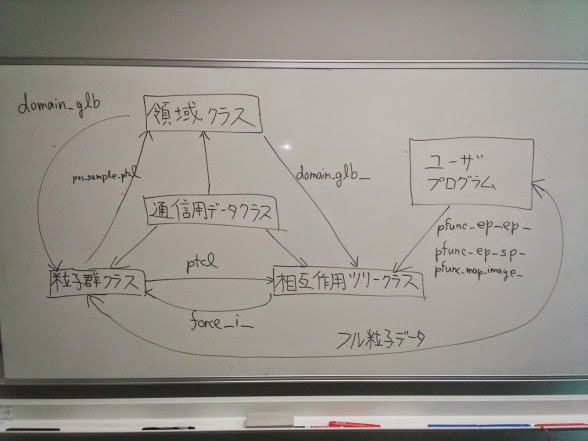
\includegraphics[width=10cm,bb=0 0 600 500]{fig/brief_interface.jpg}
    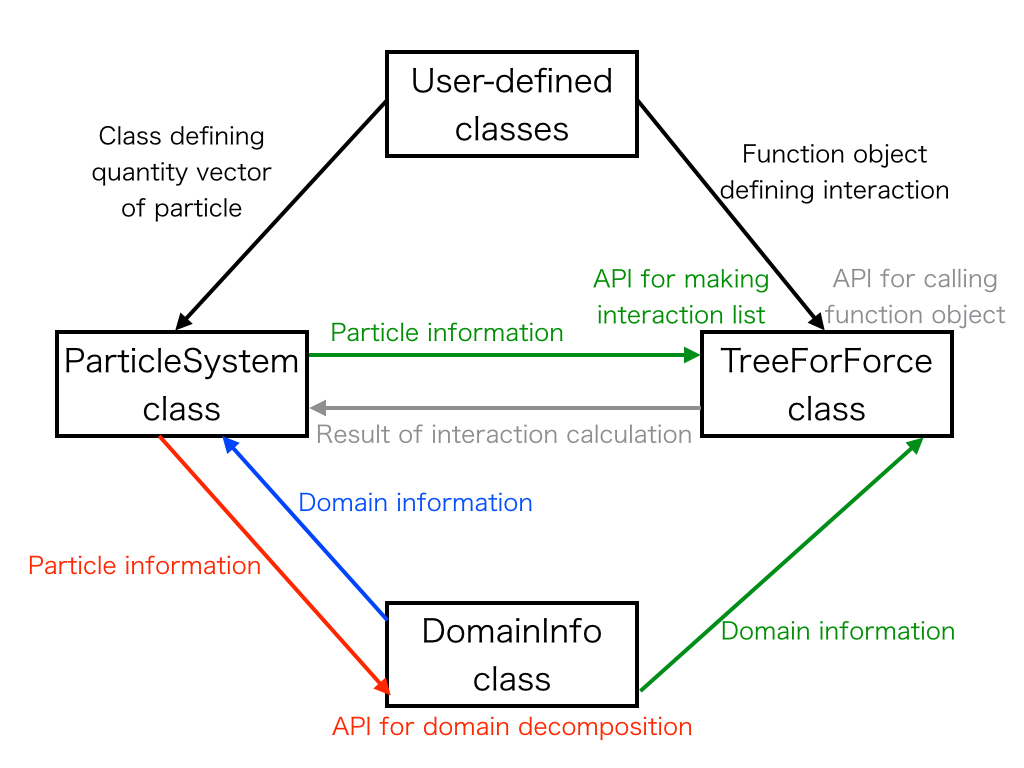
\includegraphics[width=10cm,bb=0 0 700 700]{fig/illustration/illustration.001.jpg}
  \end{center}
%%  \caption{モジュールインターフェースと情報の流れの模式図。}
  \caption{Illustration of module interface and data transfer.}
  \label{fig:brief_interface}
\end{figure}
